\subsubsection{Mining on manifolds}\label{subsec:mining_manifolds} % cooler approach

% TODO: Wie findet man manifolds?

\citet{mining_manifolds_2018} combines different definitions of proximity to mine 
for hard positives and negatives as displayed in \autoref{fig:mining_manifolds_vis}.
Given an anchor, the neighbours on the same manifold which are not neighbours in terms of 
Euclidean proximity are considered positive samples.
These positive samples should be embedded closer to the anchor in the Euclidean space.
Negative samples, on the other hand, are neighbours in the Euclidean space, 
but on different manifolds.
These samples should be embedded further away from the anchor in the Euclidean space.
The hard samples are mined from an unordered set of \textit{relevant} samples.

\begin{figure}[h]% h = here, t = top, b = bottom, p = page of floats
    \centering
    \subfloat[\centering Euclidean $k$ nearest neighbour $NN^e_k$ (orange).]
    {{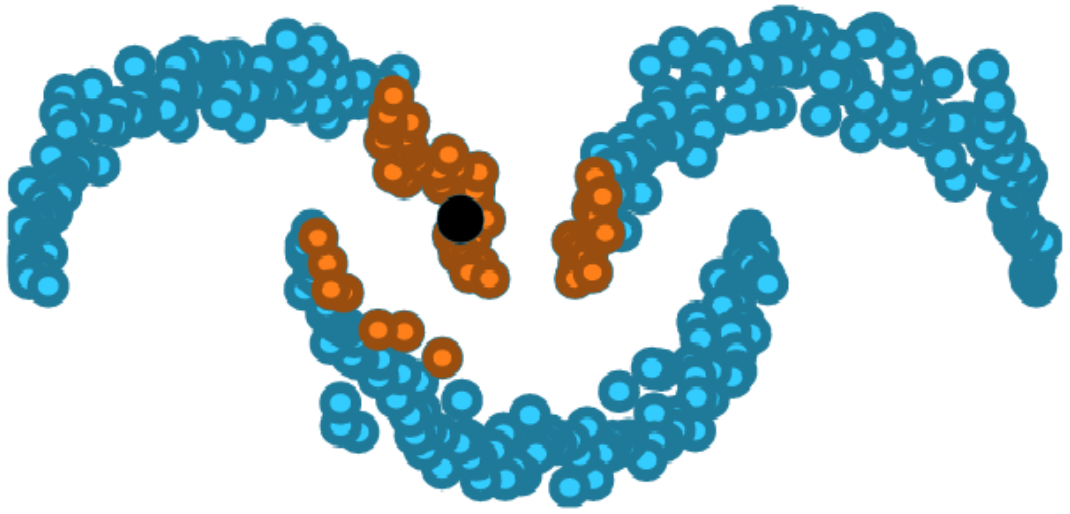
\includegraphics[width=5cm]{images/euclidean_NN.png} }}%
    \qquad
    \subfloat[\centering Manifold $k$ nearest neighbour $NN^m_k$ (purple).]
    {{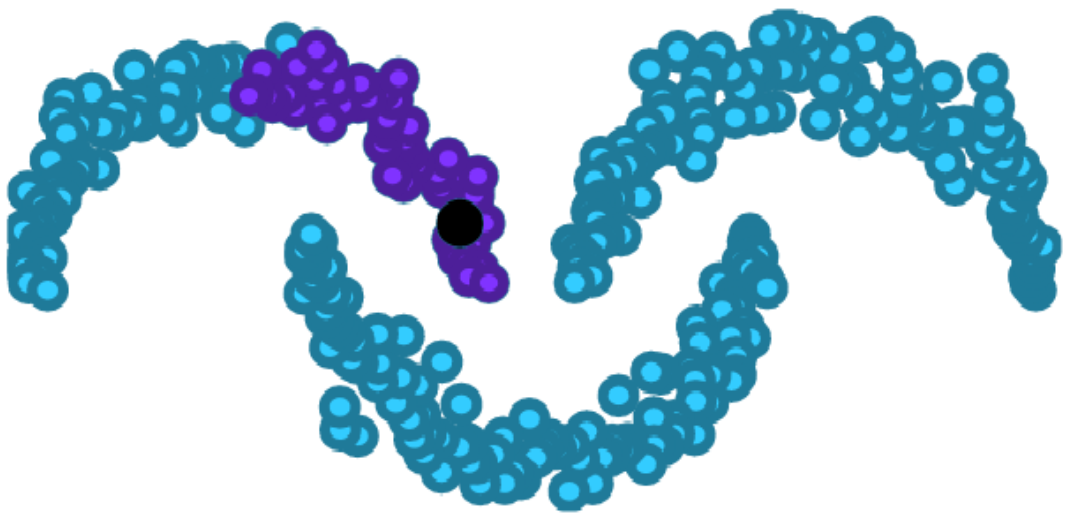
\includegraphics[width=5cm]{images/manifold_NN.png} }}%
    \qquad
    \subfloat[\centering Hard positives $NN^m_k \textbackslash NN^e_k$(green).]
    {{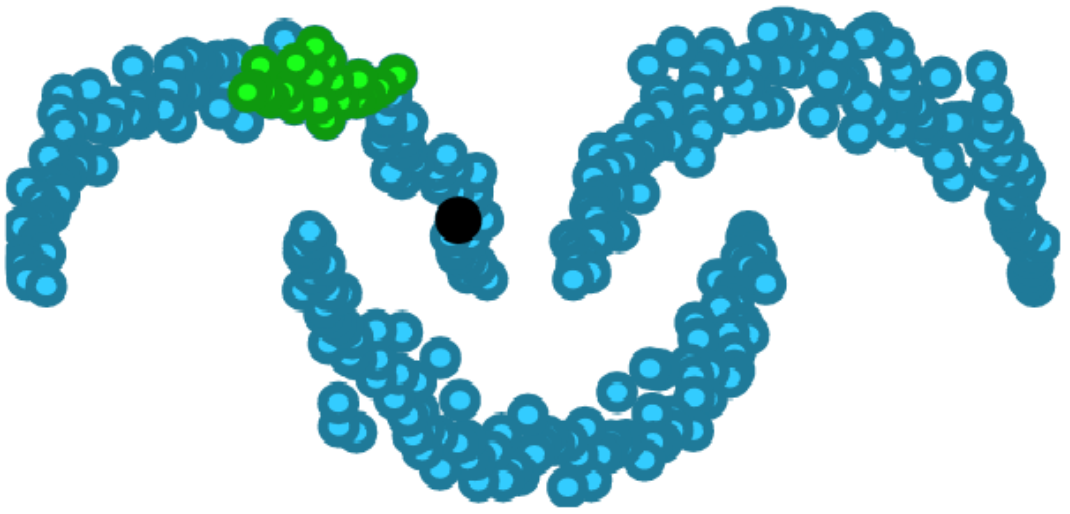
\includegraphics[width=5cm]{images/hard_positives_manifold.png} }}%
    \qquad
    \subfloat[\centering Hard negatives $NN^e_k \textbackslash NN^m_k$(red).]
    {{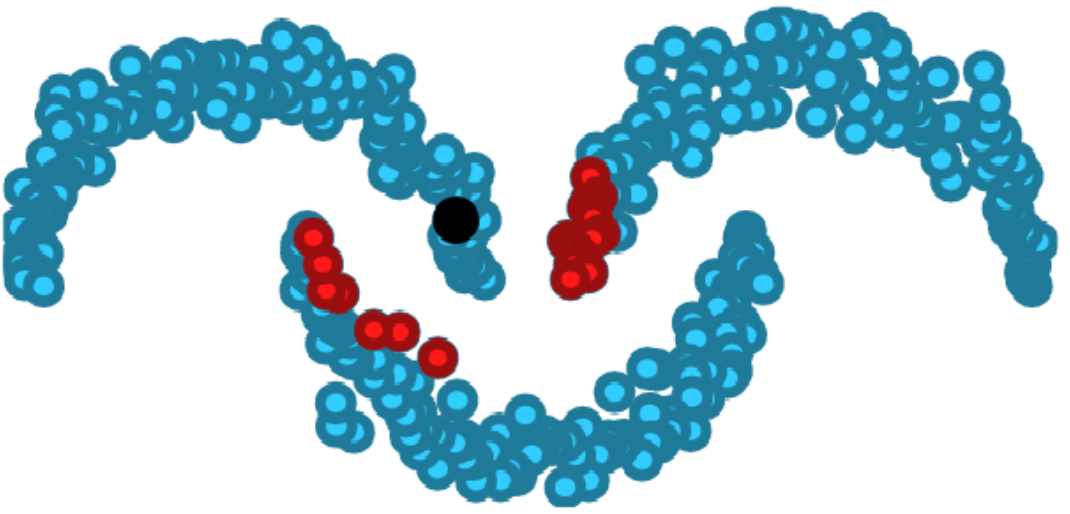
\includegraphics[width=5cm]{images/hard_negatives_euclidean.png} }}%

    \caption{Visualization of different proximity definitions and 
    the hard negatives/positives from \citet{mining_manifolds_2018}.
    The anchor is the black point.}%
    \label{fig:mining_manifolds_vis}%
\end{figure}

The authors define the $k$ nearest Euclidean neighbour $NN^e_k$ and 
the $k$ nearest manifold neighbour $NN^m_k$.
The hard positives are defined as $NN^m_k \textbackslash NN^e_k$. 
The pool $NN^m_k$ is ordered by descending manifold similarity to the anchor
to ensure that high-confidence samples are chosen first.
$k$ controls the visual diversity of the hard positives.
The larger $k$ is, the more diverse, i.e. hard, the hard positives are. 
The pool of hard negatives is defined as $NN^e_k \textbackslash NN^m_k$.
$NN^e_k$ is ordered by descending Euclidean distance to the anchor to keep the hardest samples.

% selection of anchors
\textcolor{red}{soll ich das ausführlicher beschreiben? Ja, <0.5 Seiten Formeln\\}
The anchors are selected such that they are diverse and relevant 
exploiting the structural properties of the data and the method.
This process is described in more detail in \citet{mining_manifolds_2018}.

% loss functions
\textcolor{red}{soll ich das ausführlicher beschreiben? Ja\\}
The authors propose multiple loss functions to train the model.
They, for instance, apply the contrastive loss, the triplet loss, 
and weighted versions of both contrastive and triplet loss.

% examples
\textcolor{red}{weg?\\}

% TODO: Wie positives generiert?
\begin{figure}[h] % h = here, t = top, b = bottom, p = page of floats
    \centering
    \includegraphics[width=360pt]{images/mining_manifold_qualitative_analysis.png}
    \caption{Illustration from \citet{mining_manifolds_2018}.
    The anchor is denoted $x^r$.
    A selection of hard positives from $P^+(x^r)$ is compared to the 
    baseline approach by sampling from the closest neighbours to $x^r$ in 
    terms of Euclidean distance.
    Analogously, a selection of hard negatives from $P^-(x^r)$ 
    is compared to the baseline $X \textbackslash NN^e_3$, 
    i.e. sampling from the set that contains all samples but the three closest ones in 
    terms of Euclidean distance.
    The borders of the images denote the ground-truth class.
    Green borders mean that the image belongs to the same class as the anchor,
    whereas red denotes different class images.
    It becomes apparent that the sampled hard positive consist of fewer false positives 
    as the baseline.
    }
    \label{fig:manifold_mining_qualitative_analysis}
\end{figure}

% TODO: Wie positives generiert? Wie ist eine Klasse definiert?
\begin{figure}[h] % h = here, t = top, b = bottom, p = page of floats
    \centering
    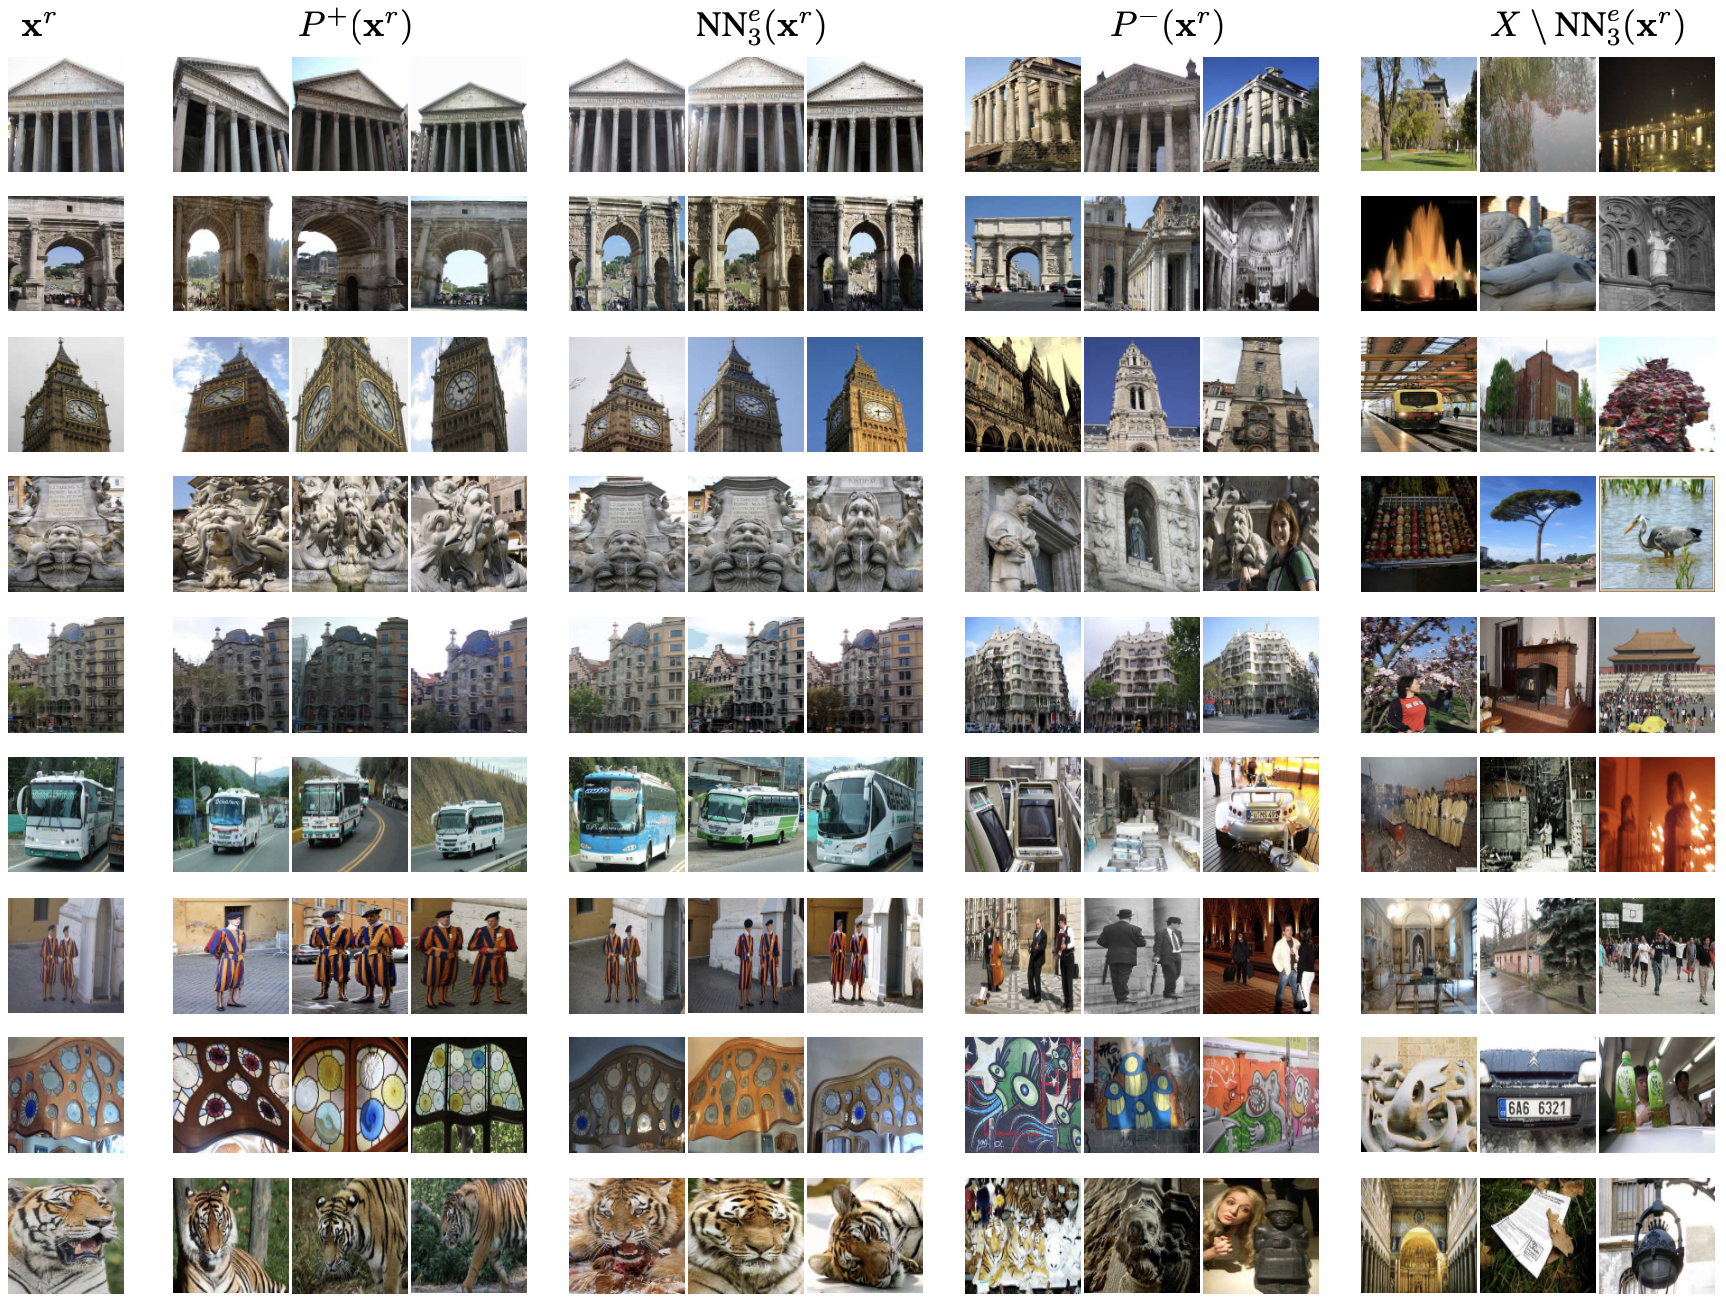
\includegraphics[width=360pt]{images/mining_manifold_examples.png}
    \caption{Illustration from \citet{mining_manifolds_2018}.
    The anchor is denoted $x^r$.
    A selection of hard positives from $P^+(x^r)$ is compared to the 
    baseline approach by sampling from the closest neighbours to $x^r$ in 
    terms of Euclidean distance.
    Analogously, a selection of hard negatives from $P^-(x^r)$ 
    is compared to the baseline $X \textbackslash NN^e_3$, 
    i.e. sampling from the set that contains all samples but the three closest ones in 
    terms of Euclidean distance.
    It becomes apparent that the hard negatives display visually similar but 
    semantically images to the anchor. % good
    }
    \label{fig:manifold_mining_examples}
\end{figure}